% o \label{codigo} serve para podermos fazer referencias para algo numerado, 
% como capitulos, tabelas, figuras, etc. 
% Quando colocamos o comando \ref{codigo}. o compilador troca o \ref{codigo}
% pelo numero atribuido ao \label{}
% ex. \label{tabelaLegal}
%   A tabela \ref{tabelaLegal} mostra que...
% vai ser substituido por
%   A tabela 2 mostra que

\chapter{Metodologia}\label{cap-metodologia}

A metodologia empregada na realização deste projeto foi o processo iterativo de design do Ciclo Formal \cite{schell:2010:art_game_design}, um método que alia conceitos de desenvolvimento ágil advindos da engenharia de software com noções modernas de game design. A adoção desta metodologia se deu pelo seu enfoque em frequentes testes e rápida iteração sobre o projeto, processos imprescindíveis no desenvolvimento de um jogo que atenda aos critérios educacionais estabelecidos, no limitado escopo estipulado.

No contexto deste projeto, a aplicação do Ciclo Formal pode ser descrita nos termos de duas etapas principais: formulação do problema e implementação iterativa.

% ---
\section{Formulação do problema}\label{sec-met-formulacao-problema}
% ---

Na etapa inicial de criação do projeto, é necessário enunciar cuidadosamente a problema a ser resolvido, levando em consideração os objetivos do jogo, sua demografia e o contexto em que ele será jogado. Também é necessário analisar os recursos disponíveis e o prazo para a criação do produto final, afim de definir um escopo claro para o projeto. A partir do levantamento dessas informações, tem-se os parâmetros a serem usados nas próximas etapas de criação do projeto.

Este problema é documentado na forma de um \textit{Game Design Document} (GDD), que servirá tanto como um relatório quanto como um ponto de referência para a realização do projeto nas etapas seguintes.


% ---
\section{Implementação iterativa}\label{sec-met-implementacao-iterativa}
% ---

Para a implementação do jogo em si, adota-se a metodologia de design iterativo, consistente de uma aplicação do ciclo de desenvolvimento de software de Boehm (\ref{fig:ciclo-boehm}) no âmbito de projetos de jogos digitais.

\begin{figure}[ht]
	\centering
	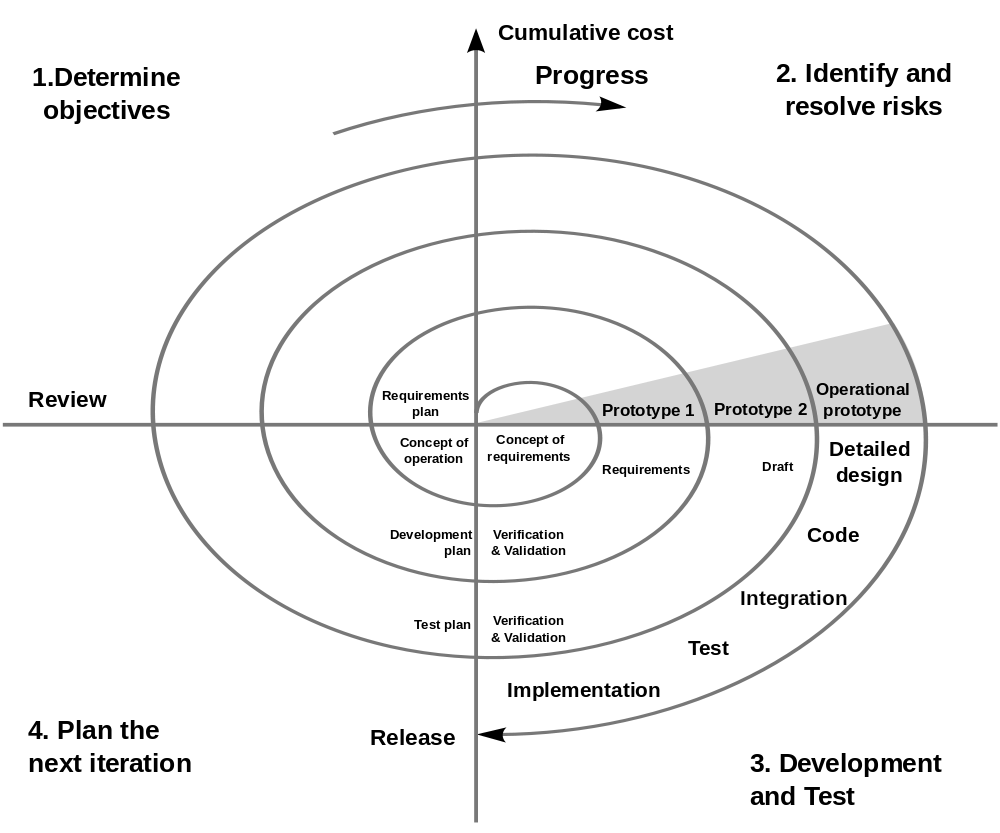
\includegraphics[width=0.5\textwidth]{ciclo_boehm}
	\caption{Ciclo de Boehm. Fonte: \cite{schell:2010:art_game_design}}
	\label{fig:ciclo-boehm}
\end{figure}

Nos termos dessa metodologia, um jogo digital deve ser implementado por meio de um processo iterativo, ciclando entre seis fase principais:

% ---
\subsection{Brainstorming}\label{subsec-met-brainstorming}
% ---

Nesta fase são propostas diversas potenciais soluções para o problema enunciado, com um enfoque na geração rápida do maior número possível de ideias, sendo evitado levantar críticas. As propostas são então listadas para avaliação quanto a seus méritos e adequação frente ao problema original elaborado, dentre as quais uma será eleita como o conceito do jogo, aprofundada e descrita formalmente em maiores detalhes.

\subsection{Escolha da solução}\label{subsec-met-escolha-solucao}

Uma das soluções propostas é escolhida, de acordo com sua aderência ao problema enunciado e viabilidade técnica. Sua descrição é então adicionada ao GDD, detalhando as características mecânicas, estéticas e tecnológicas. Esta descrição deverá ser tomada como referência para a implementação do jogo, e alterada conforme necessário durante as fases seguinte.

\subsection{Análise de riscos}\label{subsec-met-analise-riscos}

Durante a análise de riscos, um elemento específico do design deve ser considerado. Os potenciais riscos e dificuldades de implementação associados a esse segmento devem então ser levantados e listados, considerando as dinâmicas que pretende-se que esse elemento gere, sua aderência aos objetivos estipulados e eventuais problemas técnicos advindos de seu desenvolvimento.

\subsection{Prototipação}\label{subsec-met-prototipacao}

Nesta fase, procura-se elaborar rapidamente um protótipo que funcione como prova de conceito para o elemento recortado na fase anterior, de forma a eliminar ou mitigar os riscos observados. A ênfase deve ser na velocidade de implementação do protótipo, não em seu polimento ou reusabilidade dos recursos gerados em etapas posteriores do projeto.

\subsection{Teste}\label{subsec-met-teste}

Na fase de testes, o protótipo construído é avaliado quanto aos riscos delimitados na fase 3. A abrangência dos testes, variará de acordo com a natureza do elemento sendo testado e o atual estado de desenvolvimento do projeto como um todo, sendo que em testes realizados em projetos em etapas mais avançadas de seu desenvolvimento pedirão maior envolvimento de parcelas representativas do público alvo do produto final.

A adequação do elemento considerado aos objetivos esperados e sua eficácia na resolução dos problemas levantados determinarão o rumo das demais iterações do proceso.

\subsection{Análise e refinamento do design}\label{subsec-met-analise-refinamento}

Durante esta fase, uma análise das fases anteriores deve ser feita, procurando-se ressaltar os motivos que levaram a eventuais inadequações do protótipo executado aos riscos previamente delimitados. Com base nos resultados observados, as modificações necessárias são feitas ao GDD, uma nova descrição do problema é redigida, e retorna-se à fase 1 para a construção de um novo protótipo com um maior grau de polimento.

Seguindo este método, o jogo toma forma gradativamente, através de iterações e prototipações sucessivas e aditivas, até que sua implementação esteja de acordo com o estado atual do GDD, e todos os objetivos definidos tenham sido atingidos.
